\documentclass[11pt,a4paper]{article}

% Compile with LuaLaTeX. The page geometry, type size, spacing, and headings
% are chosen to make page density close to the corresponding Word template.
\usepackage[margin=1in,headheight=15pt,headsep=24pt,footskip=28pt]{geometry}
% Template specifies Source Sans Pro; use Source Sans 3 when available, else Arial.
\usepackage{fontspec}
\IfFontExistsTF{Source Sans 3}{%
  \setmainfont{Source Sans 3}%
  \setsansfont{Source Sans 3}%
}{%
  \setmainfont{Arial}%
  \setsansfont{Arial}%
}
\usepackage{setspace}
\usepackage{xcolor}
\usepackage{mdframed}
\usepackage{titlesec}
\usepackage{fancyhdr}
\usepackage{lastpage}
\usepackage{graphicx}
\usepackage{booktabs}
\usepackage{tabularx}
\usepackage{siunitx}
\usepackage{placeins}
\usepackage{float}
\usepackage[hidelinks]{hyperref}
\usepackage[numbers,sort&compress]{natbib}
\renewcommand{\bibsection}{\unnumberedheading{\refname}}

\definecolor{guidancetext}{HTML}{595959}
\definecolor{guidancebg}{HTML}{F1F3F5}

\setstretch{1}
\setlength{\parindent}{0pt}
\setlength{\parskip}{8pt}
\raggedbottom

\titleformat{\section}
  {\fontsize{14}{16.5}\selectfont\bfseries}
  {\thesection}{1em}{}
\titlespacing*{\section}{0pt}{6pt}{4pt}
\titleformat{\subsection}
  {\fontsize{13}{15.5}\selectfont\bfseries}
  {\thesubsection}{1em}{}
\titlespacing*{\subsection}{0pt}{6pt}{2pt}

\newcommand{\unnumberedheading}[1]{%
  \par\vspace{2pt}{\fontsize{14}{16.5}\selectfont\bfseries #1\par}\vspace{6pt}%
}
\newcommand{\reporttitle}[1]{%
  {\fontsize{16}{19}\selectfont\bfseries #1\par}\vspace{12pt}%
}

\pagestyle{fancy}
\fancyhf{}
\renewcommand{\headrulewidth}{0pt}
\renewcommand{\footrulewidth}{0pt}
\fancyhead[L]{\fontsize{9}{11}\selectfont II2202, Autumn 2026, Period 1}
\fancyhead[C]{\fontsize{9}{11}\selectfont Final report}
\fancyhead[R]{\fontsize{9}{11}\selectfont 2 October 2026}
\fancyfoot[R]{\fontsize{8.5}{10}\selectfont \thepage\ (\pageref{LastPage})}

\begin{document}
\reporttitle{Transparent Multi-Hop Routing for Raft Under Partial Network Partitions}
\unnumberedheading{Authors}
Lorenzo Deflorian <ldef@kth.se>\par
Juozas Skarbalius <juozas@kth.se>\par
\vspace{2pt}

\unnumberedheading{Abstract}
Raft is a leader-based consensus protocol that commits client entries only when a majority of replicas can exchange messages. Under \emph{partial} network partitions, some direct links fail while residual multi-hop paths remain. Because Raft assumes direct point-to-point communication, a leader may lose its quorum even when the network graph is still connected. Transparent multi-hop routing has been proposed as a network-layer remedy, but prior work has not experimentally characterised its effect on Raft liveness and commit latency.

We evaluate HashiCorp Raft in Mininet under five predefined topologies (healthy baseline, non-critical cut, quorum-loss, constrained election, and chained connectivity), comparing direct-only communication with preconfigured Linux multi-hop forwarding at per-link delays of \(0.5\) and \(5\,\mathrm{ms}\) (heartbeat \(10\,\mathrm{ms}\)). Across \(117\) validated trials on an AWS fleet, forwarding restores progress in the constrained-election topology where direct communication never recovers (recovery \(\approx 21\,\mathrm{s}\), then \(\approx 55\)--\(59\) commits/s), and roughly doubles observe-window throughput under quorum-loss at \(5\,\mathrm{ms}\) (\(95.3\) vs.\ \(40.1\) entries/s). When routed followers are needed for the deciding majority, median commit latency rises by about \(24\)--\(124\%\); when a direct quorum remains, the latency overhead is small (\(\leq 10\%\)). A \(20\,\mathrm{ms}\) delay with a \(10\,\mathrm{ms}\) heartbeat largely prevents stable warm-up, exposing a delay--timeout interaction. The results support transparent forwarding as an effective, protocol-preserving resilience mechanism for selected partial partitions, at a measurable latency cost when forwarded paths decide commits.

\newpage

\section{Introduction}

\subsection{Background and Rationale}

Distributed databases, file systems, and cluster orchestration services rely on consensus to agree on a shared state.
Raft is a leader-based protocol: the leader appends client entries and replicates them to followers, and an entry is committed once a majority has stored it~\cite[Sec.~5.3]{ongaro2014raft}. 
Progress requires that a leader communicates with a majority of followers. Safety is ensured under arbitrary message delay~\cite[Secs.~5.3--5.4]{ongaro2014raft}.

Complete network partitions are well understood---as long as there exists a majority of nodes that can communicate with each other, the entries can be committed.
\emph{Partial} partitions are different---individual links fail while nodes remain virtually reachable through intermediate nodes~\cite[Sec.~2]{alfatafta2020nifty}. 
Raft assumes direct point-to-point communication and does not forward messages through intermediates~\cite[Secs.~5.1--5.3]{ongaro2014raft}. 
A leader that loses two direct follower links may therefore stall even though those followers remain reachable at the network layer. 
If consensus protocol (e.g., Raft) fails to handle such partial partition topologies, it can lead to a situation where the leader is unable to commit entries, even though the network layer allows for communication between the majority of nodes.
Most notable example in this situation was observed in Cloudflare outage in 2020 [cite cloudflare blog].

This creates a mismatch between what consensus protocol considers reachable and what the network layer considers reachable during partial partitions.
This mismatch motivates asking whether transparent multi-hop routing during such partial partitions can restore Raft's progress, and at what latency cost.

\subsection{Theory and Related Work}

Jensen et al.\ studied etcd's Raft under partial failures and observed election instability and delayed requests.
They have suggested two possible solutions in the face of partial partitions: the use of \emph{PreVote} mechanism and the network overlay routing ~\cite[Secs.~5]{jensen2021raft}.
PreVote mechanism is an additional safety check in Raft where a node checks whether it could still become a leader before invoking a real election.
This prevents disrupting the cluster during partial partitions. However, they claim that PreVote substiantially increases the commit latency during partial network partitions ~\cite[Secs.~5]{jensen2021raft}. 
They suggested that the overlay networks might be a better solution in terms of reduced commit latency during partial partitions~\cite[Secs.~4--5]{jensen2021raft}. 
However, they did not evaluate the overlay networks in a systematic way.

Alfatafta et al.\ introduced Nifty, a transparent layer that re-routes traffic around failed paths. 
Nifty masks partial partitions with low overhead in several production systems such as Apache Kafka, but not Raft~\cite[Secs.~6--7]{alfatafta2020nifty}. 
They find that Nifty can restore progress with little overhead in case of partial network partition topologies.
OmniPaxos instead changes consensus itself to handle partial connectivity, and notes that overlay routing may add hops and delay~\cite[Secs.~2,8]{ng2023omnipaxos}. 
The most notable notion introduced by Omnipaxos is the majority quorum connectivity requirement during the leader election process.
They also suggest network overlays as an alternative for handling partial partitions, however they assume that the use of overlay might increase the commit latency~\cite[Secs.~2,8]{ng2023omnipaxos}.

More recent work explores protocol-level remedies. 
HoliPaxos integrates failure detection with MultiPaxos and suppresses leader churn, evaluating partial partitions against OmniPaxos and Raft with and without PreVote and CheckQuorum ~\cite[Secs. 3.1, 4.3]{liang2025holipaxos}. 
RaftOptima modifies Rafts election behaviour to limit repeated elections and introduces proxy leaders for replication scalability ~\cite[Secs. IV-V]{kondru2024raftoptima}[6, Secs. IV–V]. 
Qsync addresses partial partition livelock in leaderless Rabia consensus protocol through request queue synchronization ~\cite[Secs. 4-5]{kida2026qsync}. 
Complementary work provides automated partition testing through Slicify ~\cite{khaleel2024slicify} and probabilistic analysis of communication loss and Raft latency ~\cite{li2026consensusnetwork}.

These studies establish both the importance of partial connectivity and the availability of protocol-specific remedies.\
However, the reviewed work does not systematically characterize overlay routing beneath an unchanged Raft protocol: which partial-connectivity topologies permit progress to be restored, and how detour delay interacts with election timeouts and commit latency. 
This study targets this narrower gap.
\subsection{Research Problem, Aim, and Research Questions}

\textbf{Research problem.}
The liveness benefit and commit latency cost of applying network-layer multi-hop routing to Raft have not been experimentally characterized.

\textbf{Aim.}
Experimentally characterize transparent multi-hop routing as a network-layer resilience mechanism for Raft under a defined set of partial-connectivity topologies, in terms of liveness and commit latency, without changing the consensus implementation itself.

\textbf{Research questions.}
\begin{enumerate}
  \item \textbf{RQ1 (Liveness):} Across topologies T1--T4, in which cases does transparent multi-hop routing restore stable progress in Raft compared with direct communication only?
  \item \textbf{RQ2 (Latency):} How does added multi-hop overlay affect client-observed commit latency?
\end{enumerate}

\textbf{Hypotheses.}
\begin{enumerate}
  \item \textbf{H1:} Network overlay restores progress during partial partitions in topologies where leader still can reach majority quorum via intermediate nodes.
  \item \textbf{H2:} Commit latency increases during partial partitions where leader needs to reach majority quorum via intermediate nodes. During normal operation, little to no latency overhead is expected.
\end{enumerate}

\section{Research Method}

\subsection{Research Design and Methodological Rationale}

We answer both research questions with a controlled quantitative experiment in an emulated network.
Both RQs require paired comparisons under the same Raft implementation, failed links, workload, and timing so that differences can be attributed to communication mode and path delay.
Performing repetitions on each condition should account for election timing, network scheduling, and other noise.

The design is a comparison of communication mode (\(\mathrm{direct}\) vs.\ \(\mathrm{forwarding}\)) across five predefined topologies (T0--T4) and selected per-link delays.
T0 is a healthy baseline and T1 a control in which the leader retains a direct majority after a non-critical cut. T2--T4 instantiate quorum-loss, constrained election, and chained connectivity.
For RQ1, we observe whether commit progress is maintained or recovered after failure injection in each topology under both modes.
For RQ2, we compare client commit latency when a forwarded path is needed for the deciding majority with control cases that retain a direct quorum.
This structure matches the questions directly: topologies identify \emph{when} forwarding restores liveness, and delay levels quantify the latency cost of the extra hop.

We considered several alternatives and rejected them as less suitable for the stated questions.
First, adaptive overlays such as Nifty combine failure detection, route discovery, and forwarding~\cite{alfatafta2020nifty}.
Using Nifty would have confounded the effect of multi-hop path availability with discovery and installation latency. Instead, use minitet so that the treatment is path availability and delay alone.
Second, protocol-level remedies (PreVote, Omni-Paxos-style quorum connectivity, HoliPaxos) change consensus behaviour rather than the network underneath an unchanged Raft~\cite{jensen2021raft,ng2023omnipaxos,liang2025holipaxos}.
Those approaches answer a different question. Our aim is to evaluate a network-layer remedy without modifying the consensus implementation.
Therefore we opted out for executable Mininet deployment for network emulation with HashiCorp Raft for consensus cluster~\cite{hashicorp_raft,lantz2010mininet}.

We assume that preconfigured forwarding correctly realizes the intended network topology (T0--T4), that Mininet link delay overhead is negligible compared to artificial per-link delay, and that client observed latencies are sufficient for measuring commit latency.
We constrain the study to HashiCorp Raft with a fixed heartbeat (\(10\,\mathrm{ms}\)), an open-loop client (\(100\) requests/s, \(64\,\mathrm{B}\) payloads), and a short observation window (\(30\,\mathrm{s}\)).

Relative to the research plan, the methodological core---controlled Mininet experiment, direct vs.\ preconfigured forwarding, topologies T0--T4, and delay factors---is unchanged.
Two practical changes were made.
The plan intended to run all trials on a single personal machine. To execute all experiments within the course deadline we moved execution to AWS EC2 instances, with each instance uploading Raft logs, client logs, and metrics to S3 for later merge.
We also fixed the heartbeat at \(10\,\mathrm{ms}\) rather than testing against multiple heartbeat values, so that delays can be interpreted against one baseline heartbeat value.
These changes preserve original research intentions while adapting to existing resources and time constraints.

\subsection{Experimental Platform and Conditions}

Evidence comes from timed Mininet trials of HashiCorp Raft~\cite{hashicorp_raft,lantz2010mininet,mininet230} under fixed topology, mode, and delay, with an open-loop client (\(100\) requests/s, \(64\,\mathrm{B}\)).
There are no human participants or personal data.
In direct mode, replicas use surviving point-to-point links; in forwarding mode, preconfigured Linux routes carry the same peer addresses over multi-hop paths.
Heartbeat is fixed at \(10\,\mathrm{ms}\).
Trials ran on AWS \texttt{c5a.large} workers with host-load monitoring; each instance uploaded client logs, Raft events, and metrics to S3 for merge into \texttt{dataset.jsonl}.
Commit latency uses client-side timestamps.

Figure~\ref{fig:topologies} shows topologies T0--T4 (healthy baseline, non-critical cut, quorum-loss, constrained election, chained connectivity).
Tables~\ref{tab:independent-variables} and~\ref{tab:dependent-variables} list the independent and dependent variables.

\begin{table}[htbp]
  \centering
  \caption{Independent variables.}
  \label{tab:independent-variables}
  \begin{tabular}{ll}
    \toprule
    Independent variable & Level \\
    \midrule
    Communication mode & Point-to-Point (P2P) RPC, Multi-hop RPC forwarding \\
    Topology & T0--T4 \\
    Per-link delay & 0.5, 5, 20\,ms \\
    \bottomrule
  \end{tabular}
\end{table}

\begin{table}[htbp]
  \centering
  \caption{Dependent variables.}
  \label{tab:dependent-variables}
  \begin{tabular}{lll}
    \toprule
    Dependent variable & RQ & Definition \\
    \midrule
    Commit throughput & RQ1 & Committed and appended entries per second \\
    Recovery time & RQ1 & Time from failure to first subsequent commit \\
    Number of elections & RQ1 & Count during the observation window \\
    Number of term changes & RQ1 & Count during the observation window \\
    Commit latency & RQ2 & Client request-response delay \\
    \bottomrule
  \end{tabular}
\end{table}

\begin{figure}[H]
  \centering
  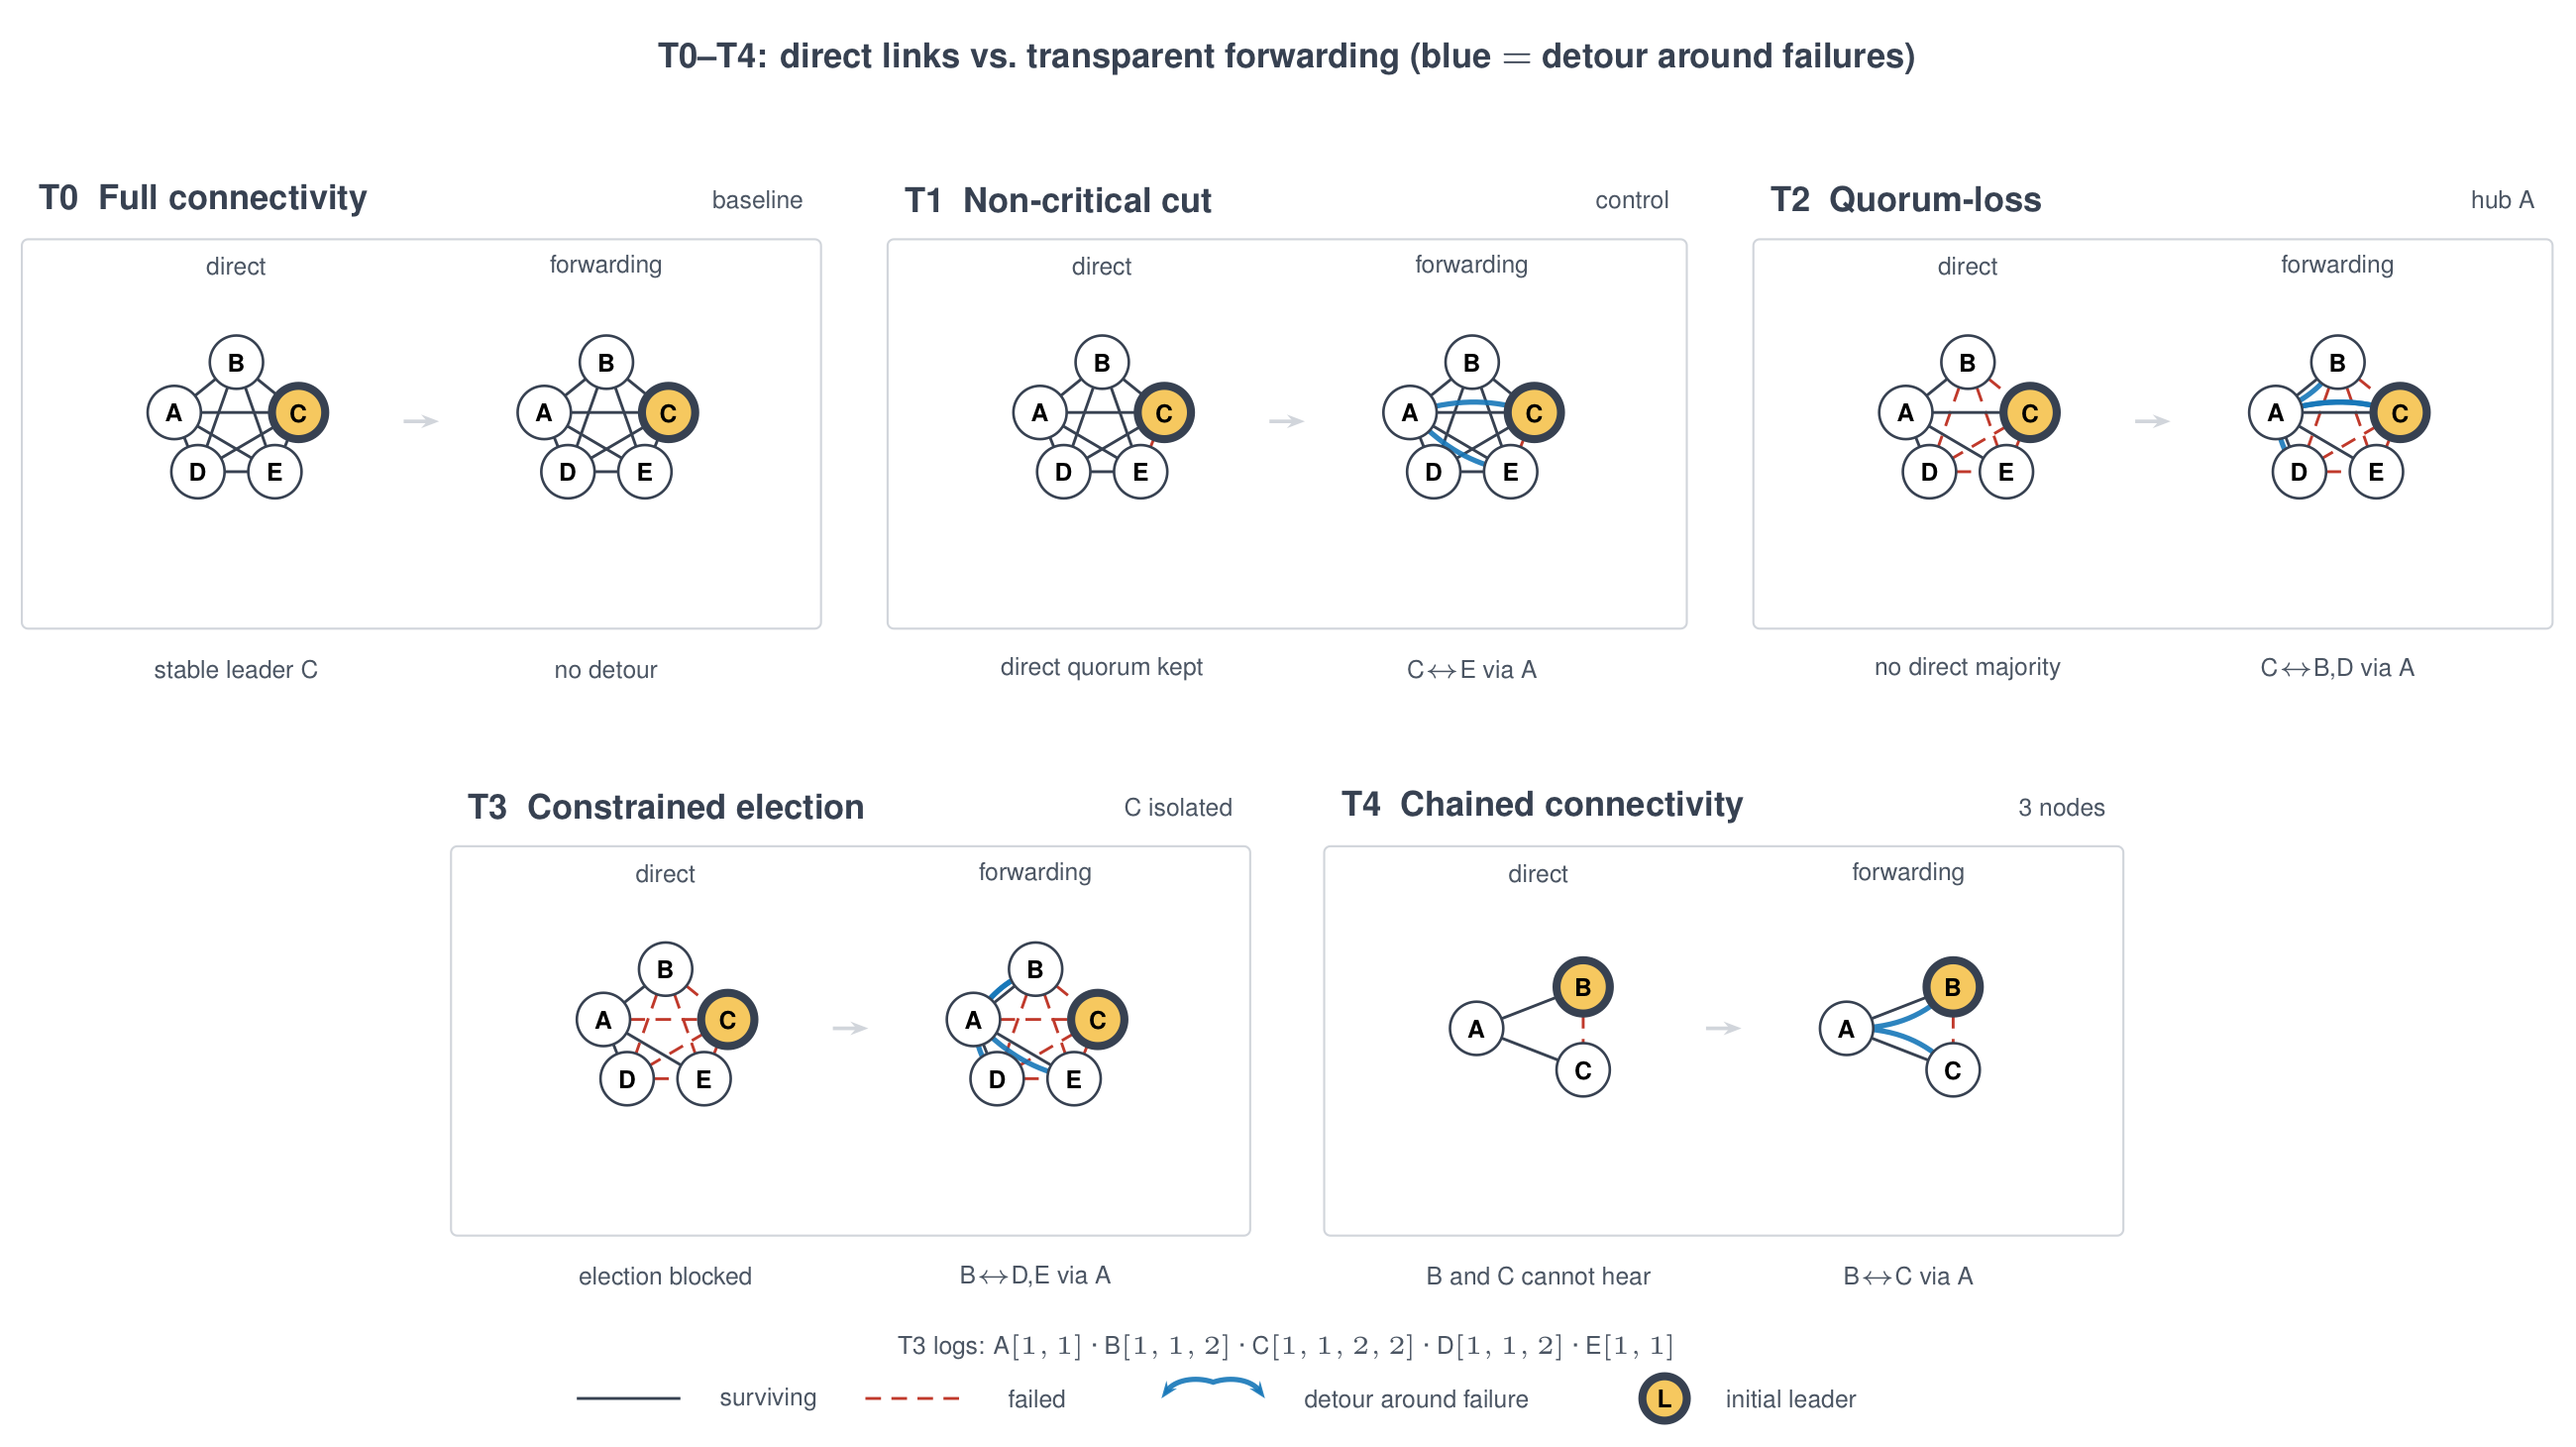
\includegraphics[width=0.92\textwidth]{figures/topology-scenarios.png}
  \caption{Direct-only vs.\ transparent forwarding. Solid links remain; dashed links fail; blue paths are forwarding over surviving links.}
  \label{fig:topologies}
\end{figure}

Of the planned \(900\) trials (\(5\times 2\times 3\times 30\)), campaign \texttt{full-20261001A} produced \(117\) validated runs, \(43\) failures (mostly \(20\,\mathrm{ms}\) warm-up failures), and \(740\) not executed.
A trial is included only if warm-up yields \(\geq 1\) commit, post-inject connectivity matches the intended residual graph, and artefacts are complete; otherwise it is excluded.
Reported cells therefore typically have \(n=5\)--\(6\), and most \(20\,\mathrm{ms}\) cells are absent from comparisons.
Interpretation is limited to this Mininet/HashiCorp setup, the five topologies, and a \(30\,\mathrm{s}\) observe window; in T4 a three-node majority is size two, so the missing \(B\)--\(C\) link is not critical for liveness under our workload.

\subsection{Work Procedure and Data Collection}
\label{sec:procedure}

Each trial follows a fixed sequence: clean Mininet topology with the chosen per-link delay; boot replicas with the planned leader and log seed; start the open-loop client; warm up \(10\,\mathrm{s}\) (require \(\geq 1\) commit); inject the topology's failed links; observe \(30\,\mathrm{s}\); archive client logs, Raft events, timeline, and host load; tear down before the next run.
Seeds are derived from base \(20260926\).
Forwarding routes and failed-link sets are taken from topology YAML so both modes share peer addresses and differ only in path availability.
Material deviations from the research plan are the AWS parallel campaign (instead of a single local VM), heartbeat fixed at \(10\,\mathrm{ms}\), target repetitions raised to \(30\) but only \(5\)--\(6\) completed per analysed cell, and exclusion of most \(20\,\mathrm{ms}\) cells after warm-up failure (T3 at \(20\,\mathrm{ms}\) completed warm-up but made no progress).
Full artefact layout and campaign counts are in Appendix~A.

\subsection{Data Analysis and Quality Assurance}

For RQ1, within each topology we compare direct vs.\ forwarding on observe-window commit throughput, recovery time (inject \(\rightarrow\) first post-failure commit), election/term counts, and client fail rate; T0/T1 are controls.
Primary claims use throughput and recovery; the boolean \texttt{stable\_progress} flag is secondary because it can label near-zero progress as stable.
For RQ2, we take the median (and 95th percentile) client commit latency per run and contrast cells where a forwarded follower is needed for the deciding majority (notably T2) with direct-quorum controls (T0/T1); when only forwarding is live (T3), latency is reported for that mode alone.
With \(n=5\)--\(6\) we report means \(\pm\)\,SD rather than formal hypothesis tests.
Validity is supported by paired conditions, fixed binaries and seeds, post-inject connectivity checks, host-load monitoring, and exclusion of invalid warm-ups; scripts, topology YAML, and \texttt{dataset.jsonl} are archived with the campaign (Appendix~A).

\subsection{Use of AI Tools}

AI tools assisted with experiment harness scripts, figure generation, grammar/style editing of the report, and structuring tables from the measurement dataset. All scientific claims, design choices, and interpretations were reviewed and verified by the authors against the raw campaign outputs.

\section{Results}

Unless noted, results refer to delays of \(0.5\,\mathrm{ms}\) and \(5\,\mathrm{ms}\) with heartbeat \(10\,\mathrm{ms}\) and \(n=5\) or \(6\) validated runs per cell (means \(\pm\)\,SD where shown).
Figure~\ref{fig:rq1-thr} summarises observe-window commit throughput; Figure~\ref{fig:rq2-lat} summarises mean per-run median commit latency.
Most \(20\,\mathrm{ms}\) cells failed warm-up and are reported separately rather than pooled with the main comparisons.

\begin{figure}[H]
  \centering
  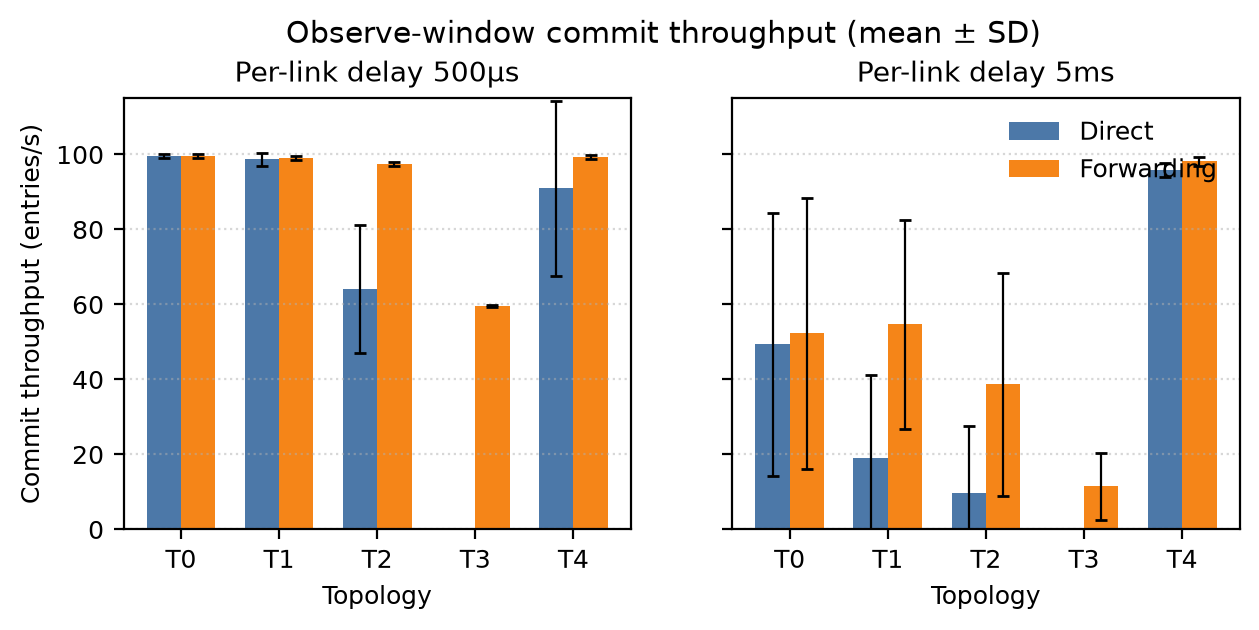
\includegraphics[width=0.95\textwidth]{figures/rq1-throughput.png}
  \caption{Mean observe-window commit throughput (\(\pm\)\,SD) by topology and mode.}
  \label{fig:rq1-thr}
\end{figure}

\begin{figure}[H]
  \centering
  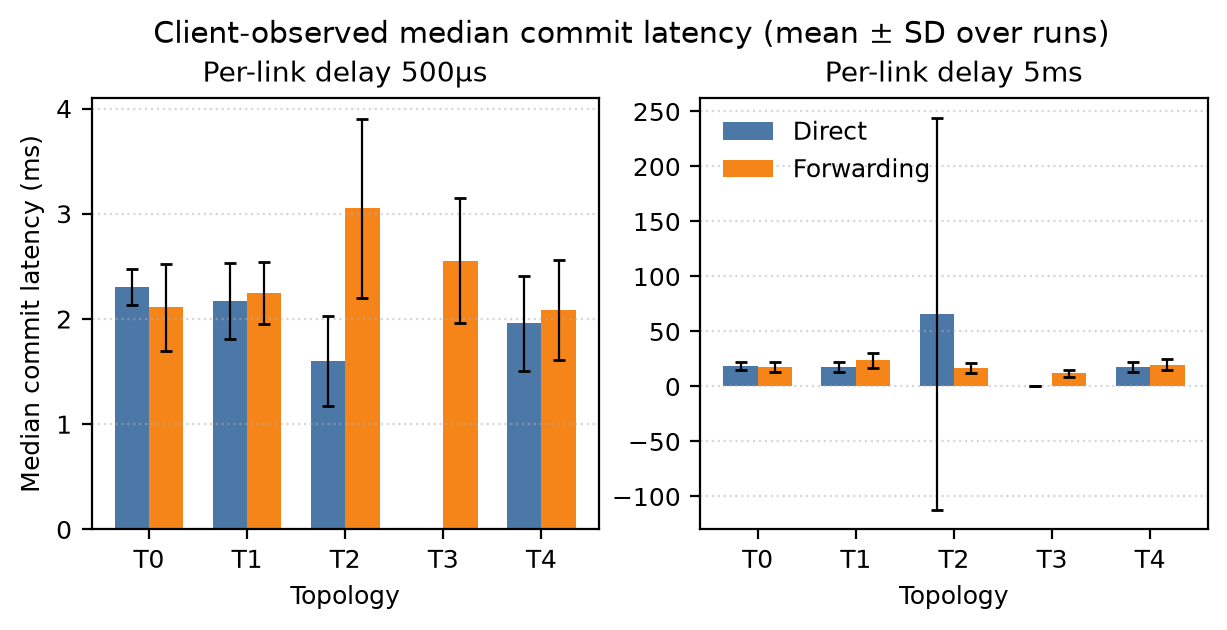
\includegraphics[width=0.95\textwidth]{figures/rq2-latency.png}
  \caption{Mean of per-run median commit latencies (\(\pm\)\,SD). Missing bars: no successful commits.}
  \label{fig:rq2-lat}
\end{figure}

\subsection{RQ1: Liveness and recovery}

\textbf{Controls (T0, T1).}
Both modes remain live: mean throughput \(\approx 98\)--\(100\) entries/s, recovery of a few milliseconds after inject, and client fail rates \(\leq 1.6\%\).
Direct and forwarding outcomes are qualitatively the same when the leader already has a direct majority.

\textbf{T2 (quorum-loss).}
At \(0.5\,\mathrm{ms}\), direct mean throughput is \(68.4\) entries/s and forwarding \(97.4\).
At \(5\,\mathrm{ms}\), forwarding sustains \(95.3\) entries/s (fail rate \(4.7\%\)), while direct averages \(40.1\) with high variance: two of five runs essentially stall (\(\approx 0.11\) entries/s, \(>3900\) client failures) and three run near \(67\) entries/s.
Forwarding is therefore associated with near-full observe-window progress in this topology; direct communication is degraded and, in some runs, nearly dead.

\textbf{T3 (constrained election).}
Direct communication never recovers at any tested delay: throughput \(0\), fail rate \(100\%\).
Forwarding at \(0.5\,\mathrm{ms}\) recovers in all five runs after \(20.5\pm 0.1\,\mathrm{s}\), then commits at \(\approx 59\) entries/s for the remainder of the \(30\,\mathrm{s}\) window (elections \(\approx 8\)).
At \(5\,\mathrm{ms}\), four of five runs recover (\(\approx 21.5\,\mathrm{s}\), throughput \(\approx 56\) entries/s) but with far more election churn (\(\approx 199\)).
At \(20\,\mathrm{ms}\), forwarding also fails and produces election storms (\(\approx 750\) elections).
Figure~\ref{fig:t3-rec} shows recovery times for the successful forwarding cases.

\begin{figure}[H]
  \centering
  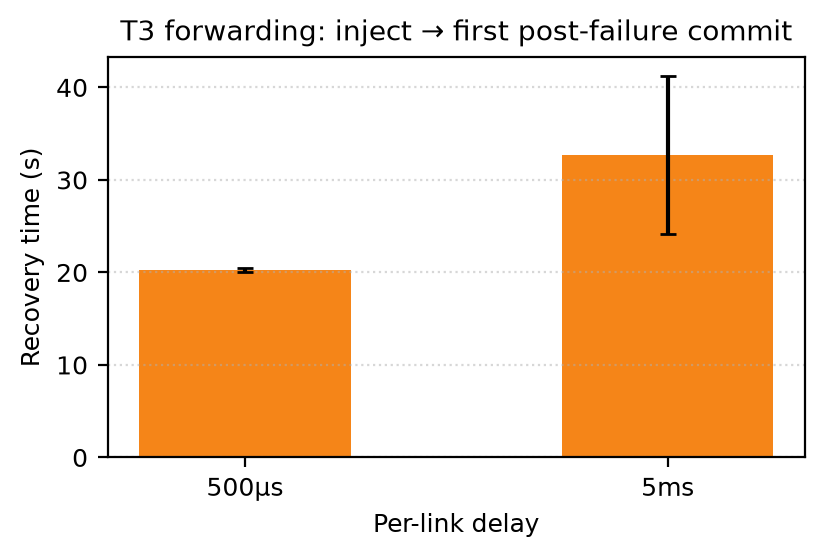
\includegraphics[width=0.48\textwidth]{figures/rq1-t3-recovery.png}
  \caption{T3 forwarding recovery time (inject to first post-failure commit).}
  \label{fig:t3-rec}
\end{figure}

\textbf{T4 (chain).}
Both modes remain live at \(\approx 98\)--\(100\) entries/s.
With three nodes, majority size is two, so leader \(B\) can commit with \(A\) alone; observe-window throughput therefore does not separate the modes under this workload.

\textbf{Warm-up failures at \(20\,\mathrm{ms}\).}
All T0/T1/T2/T4 runs at \(20\,\mathrm{ms}\) failed the warm-up commit check under heartbeat \(10\,\mathrm{ms}\) and are excluded from the throughput and latency comparisons above.
T3 at \(20\,\mathrm{ms}\) completed warm-up but made no post-inject progress under either mode.

\subsection{RQ2: Commit latency}

Table~\ref{tab:latency} reports the mean of per-run median commit latencies.
Absolute latency tracks configured per-link delay (\(\approx 2\)--\(3\,\mathrm{ms}\) at \(0.5\,\mathrm{ms}\) link delay; \(\approx 17\)--\(21\,\mathrm{ms}\) at \(5\,\mathrm{ms}\)).

\begin{table}[H]
  \centering
  \caption{Mean of per-run median commit latencies (ms). ``--'' = no successful commits.}
  \label{tab:latency}
  \footnotesize
  \begin{tabular}{llrrrr}
    \toprule
    Topology & Delay & Direct & Forwarding & Ratio & Context \\
    \midrule
    T0 & \(0.5\,\mathrm{ms}\) & 2.64 & 2.65 & 1.01 & Direct quorum \\
    T0 & \(5\,\mathrm{ms}\) & 17.33 & 18.98 & 1.10 & Direct quorum \\
    T1 & \(0.5\,\mathrm{ms}\) & 2.48 & 2.66 & 1.07 & Direct quorum \\
    T1 & \(5\,\mathrm{ms}\) & 18.97 & 18.67 & 0.98 & Direct quorum \\
    T2 & \(0.5\,\mathrm{ms}\) & 1.64 & 3.68 & 2.24 & Forwarded majority \\
    T2 & \(5\,\mathrm{ms}\) & 18.85 & 20.67 & 1.10 & Mixed direct outcomes \\
    T3 & \(0.5\,\mathrm{ms}\) & -- & 3.46 & -- & Fwd only live \\
    T3 & \(5\,\mathrm{ms}\) & -- & 14.65 & -- & Fwd only live \\
    T4 & \(0.5\,\mathrm{ms}\) & 1.75 & 2.38 & 1.35 & Extra hop available \\
    T4 & \(5\,\mathrm{ms}\) & 16.59 & 20.59 & 1.24 & Extra hop available \\
    \bottomrule
  \end{tabular}
\end{table}

When a direct quorum remains (T0/T1), the forwarding/direct ratio is \(\leq 1.10\).
When forwarded followers are needed for the deciding majority (T2 at \(0.5\,\mathrm{ms}\)), the mean of medians more than doubles (ratio \(2.24\)).
T4 shows a moderate increase (ratios \(1.24\)--\(1.35\)) even though observe-window throughput already saturates without the far endpoint.
After T3 recovers, forwarding-only latency is in the same range as other live cells at the same delay.
The T2 direct cell at \(5\,\mathrm{ms}\) remains hard to interpret as a single ratio because of the bimodal stall/progress pattern noted under RQ1.

\section{Discussion}

\subsection{Interpretation and Answers to the Research Questions}

\textbf{RQ1.}
Across T1--T4, transparent multi-hop routing restores or clearly improves post-failure progress in T2 and T3, is redundant for T1 (and the T0 baseline), and does not change the liveness outcome in T4 under a three-node majority.
H1 is supported where the residual forwarded graph gives a viable path to a majority (T2, T3), with two caveats already visible in the data: T3 recovery consumes most of the \(30\,\mathrm{s}\) observe window (\(\approx 21\,\mathrm{s}\)), and at \(5\,\mathrm{ms}\) T3 forwarding succeeds with high election churn.
T4 is a negative control for ``always rescue'': both modes already progress because \(B\) needs only \(A\).
An alternative explanation for T2's bimodal direct runs is transient scheduling or election timing rather than a stable direct quorum; the forwarding cell does not show the same stall mode at \(5\,\mathrm{ms}\).

\textbf{RQ2.}
H2 is supported in direction: latency overhead is small when a direct quorum remains (\(\leq 10\%\) in T0/T1) and large when a forwarded path participates in the deciding majority (T2 at \(0.5\,\mathrm{ms}\)).
Absolute latency is dominated by configured per-link delay.
T4's moderate overhead without a liveness difference suggests that forwarding can still lengthen some commit paths or add scheduling cost even when the far node is not required for majority.
The \(20\,\mathrm{ms}\) warm-up failures show a hard interaction: with heartbeat \(10\,\mathrm{ms}\), the cluster often never becomes initially stable, so forwarding cannot be credited or blamed for post-inject behaviour in those cells.

Relative to prior work, the results empirically support Jensen et al.'s suggestion that overlays can help Raft under partial partitions~\cite{jensen2021raft} and align with Nifty's claim that transparent detours can mask such failures~\cite{alfatafta2020nifty}, while quantifying Raft-specific recovery delay and commit-latency cost that Omni-Paxos discussed qualitatively~\cite{ng2023omnipaxos}.
Unlike Omni-Paxos or HoliPaxos, the consensus protocol here is unchanged; the trade-off is network-layer overhead and timeout co-design rather than protocol redesign.

\subsection{Validity, Limitations, and Generalizability}

Internal validity is helped by paired topologies and modes, fixed binaries, recorded seeds, post-inject connectivity checks, and host-load monitoring.
Confidence is reduced by incomplete repetitions (\(n=5\)--\(6\) instead of \(30\)), bimodal T2-direct behaviour at \(5\,\mathrm{ms}\), exclusion of most \(20\,\mathrm{ms}\) cells, and the secondary \texttt{stable\_progress} heuristic, which we therefore do not treat as primary evidence.
Construct validity for ``stable progress'' rests on throughput, recovery, elections, and fail rate rather than a single boolean.
External validity is limited to Mininet emulation, HashiCorp Raft with heartbeat \(10\,\mathrm{ms}\), the five hand-designed topologies, a \(30\,\mathrm{s}\) observe window, and AWS \texttt{c5a.large} workers.
Production WANs, larger clusters, lossy links beyond static delay, and adaptive overlays (e.g., Nifty route discovery) may differ.
Latency measurement uses client-side timestamps to avoid mixing clocks with Raft event logs; that choice improves RQ2 consistency but does not capture server-internal queueing separately.

\subsection{Ethics, Societal Aspects, and Sustainability}

The project uses open-source software and synthetic workloads only; no personal data or human participants are involved, so consent and anonymization issues do not arise.
Stakeholders who could be affected by applying the results include operators of consensus-backed services (databases, coordination, multi-homed cloud networks) and their users, for whom partial partitions threaten availability.
Transparent forwarding can improve resilience without forking Raft codebases, which may lower adoption cost, but operators must weigh added commit latency and the risk of election storms when path delay approaches heartbeat periods---misapplication could trade silent stall for prolonged leader churn.
Environmentally, the campaign used a short eight-instance AWS fleet; failed and incomplete cells still consumed energy, which argues for tighter warm-up/timeout co-design before repeating large matrices.
Socially, more available coordination services under partial failure can reduce outage impact, provided latency SLOs remain acceptable.

\subsection{Implications and Future Work}

Practically, static multi-hop forwarding is a viable mitigation for selected partial partitions when a \(\approx 20\,\mathrm{s}\) recovery (as in T3) and moderate latency growth are acceptable, and when timeouts are scaled to path delay.
Scientifically, the study narrows the gap between overlay proposals for Raft and measured liveness/latency under concrete topologies, while showing that chain topologies need quorum-critical far endpoints before forwarding can be credited for rescue.

If continued as a Master's project, priority next steps would be:
(i)~complete the \(30\)-repetition matrix with heartbeat and election timeouts scaled to delay, so \(20\,\mathrm{ms}\) (and higher) cells are evaluable;
(ii)~compare preconfigured forwarding with a discovery-based overlay such as Nifty to separate path benefit from detection latency;
(iii)~revisit T4-like chains in five-node settings where the far node \emph{is} required for majority;
(iv)~characterise recovery-time and election-churn distributions under varied timeouts, focusing on the T3 failure mode.

\section{Conclusion}

Under the tested Mininet/HashiCorp conditions, transparent multi-hop forwarding restores progress in the constrained-election topology (T3) and preserves near-full observe-window throughput under quorum-loss (T2), while direct communication fails or degrades in those cases.
When a direct quorum remains (T0/T1), forwarding adds little commit latency; when forwarded followers decide the majority, median latency can more than double, and T3 recovery itself is long relative to the \(30\,\mathrm{s}\) window.
T4 shows no liveness benefit under a three-node majority.
Overall, network-layer multi-hop routing is a protocol-preserving resilience option for selected partial partitions, provided Raft timeouts accommodate path delay and operators accept the measured latency and recovery costs.

\newpage
\bibliographystyle{myIEEEtran}
\bibliography{II2202-report}

\newpage
\unnumberedheading{Appendix A: Procedure detail and campaign completeness}

\textbf{Trial sequence (expanded).}
(1)~Start a clean Mininet topology for the assigned T0--T4 scenario and apply the chosen per-link delay to all surviving links.
(2)~Configure and start HashiCorp Raft replicas with the planned initial leader, log seed, and heartbeat \(10\,\mathrm{ms}\); in forwarding mode install the preconfigured Linux routes.
(3)~Start the open-loop client (\(100\) requests/s, \(64\,\mathrm{B}\)).
(4)~Warm up \(10\,\mathrm{s}\) and abort the trial if no successful commit occurs.
(5)~Inject the topology's failed links; validate residual connectivity against the intended graph for the assigned mode.
(6)~Observe \(30\,\mathrm{s}\) under the same client workload.
(7)~Stop client and replicas, archive artefacts under a unique run id, and tear down Mininet before the next trial.
Seeds are derived from base \(20260926\).

\textbf{Campaign completeness.}
Planned matrix: \(5\) topologies \(\times\) \(2\) modes \(\times\) \(3\) delays \(\times\) \(30\) repetitions \(= 900\) trials.
Campaign \texttt{full-20261001A} yielded \(117\) validated successful trials, \(43\) failed
(almost all \(20\,\mathrm{ms}\) warm-up failures on T0/T1/T2/T4), and \(740\) not executed.
Workers: AWS \texttt{c5a.large}. Analysis dataset: \texttt{experiments/viz/public/data/dataset.jsonl}.
Artefacts per successful run include \texttt{client.jsonl}, \texttt{events-*.jsonl},
\texttt{timeline.json}, \texttt{metrics.json}, and \texttt{hostload.jsonl}.
Experiment scripts, topology YAML, and forwarding rules are archived with the repository.

\unnumberedheading{Appendix B: AI tool use (summary)}

AI assistance was used for harness/script authoring, aggregating \texttt{dataset.jsonl} into tables/figures, and editorial revision of LaTeX drafts. Prompts concerned formatting, statistical summaries, and wording; no AI-generated measurement values were accepted without recomputation from campaign files. Authors remain responsible for all scientific content.
\end{document}
